\subsection{Drift System Implementation}
\label{driftimplementation}

The last chapter conceptionally introduced the \textit{Drift language}
as well as the \textit{Drift Shell}. This chapter will introduce
the current implementation of the \textit{Drift} back-end system,
based on the ideas presented so far.

Both, the Drift language and shell, are heavily influenced
by the idea that most of the semantics of programming for us
programmers is contained within the \textit{names} that are being
used. Which makes it hard to differentiate between which
functionality is defined by the language and which by the shell.

One example of this would be the variable-space which is
defined to consist of names and namespaces only, forming the same
kind of namespace-tree as a traditional UNIX file system.
This tree and variable-space can be walked using the language
keywords \texttt{ls} and \texttt{cd} which are therefor implemented
as shell built-ins.

Furthermore some assumptions and invariants of the underlying
system's behavior have also been sketched, based on the ideas
introduced by chapters \ref{LanguageOfTheSystem} - \ref{bretvictor}.
One example of this would be, that names can be removed from
the pseudo-global namespace emulated by each shell session,
but the data that is referenced by this name needs to be
held on to and made available by the system in case any
running service is still consuming from this data.
So using the concepts of Rich Hickey as introduced in
chapter \ref{LanguageOfTheSystem}, from the user perspective
names behave like places but from the system perspective
data behaves like values.

Another aspect that has already been scratched upon, is the
idea that data should be made observable as soon as it is
available. This is based on the realization that batch
processing is only a special case of stream processing.
In other words: batch data is just streaming data with all
the stream snippets that would otherwise trickle down
over time having already arrived. Therefor any system that
is able to deal with the fact that data might only arrive
as delayed chunks, will naturally be able to deal with a
delay size of 0.

So in order to build a back-end system that supports these
assumptions, one needs to first define the basic tasks of
the front-end (the shell), the back-end and how they interface
with one another. Fig.\ref{system-abstract} shows the
basic idea of how this looks in the current implementation.

\begin{figure}[h]
  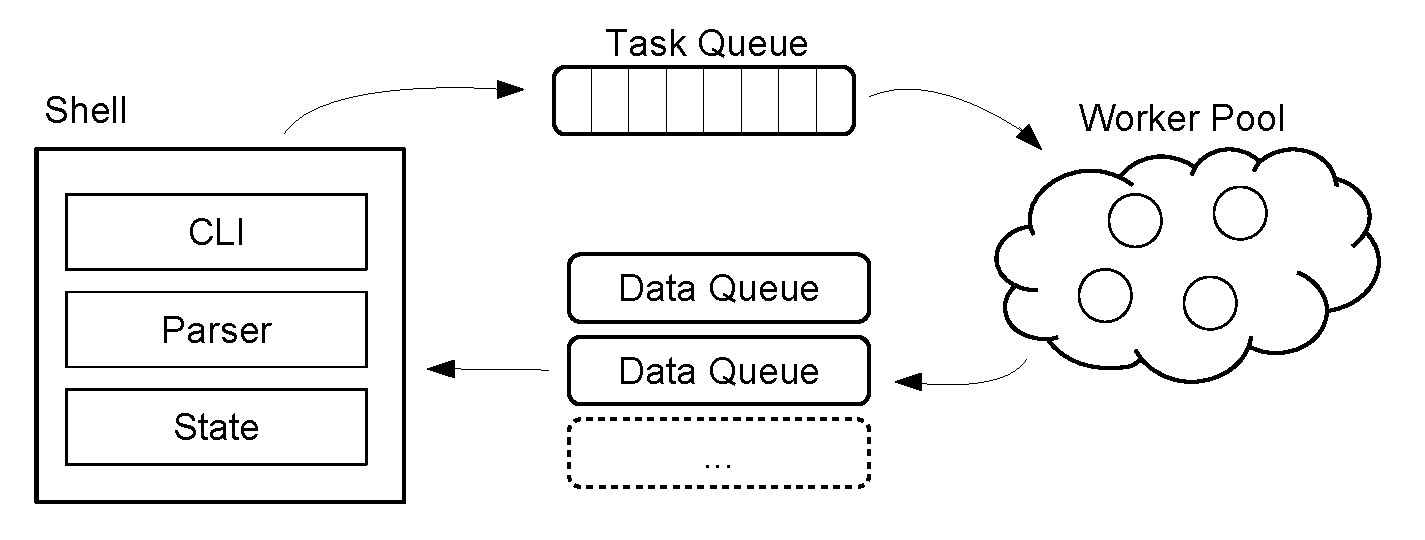
\includegraphics[scale=0.6, keepaspectratio]{system_abstract.pdf}
  \caption{Abstract architecture of the Drift front-end and back-end
           and the interfacing between the two.}
  \label{system-abstract}
\end{figure}

\subsubsection{Drift Shell}
\label{driftshell}

The shell's job is to present the user with a textual interface
and send any valid commands as tasks to the system. Therefor
the shell is \textit{not} part of the system per se. It runs
on the user's machine and connects to the system via network.
This means the user can interface with the system virtually from
anywhere.
This might seem insignificant but another vital task of
the shell is to present the user with its own
seperated and stateful environment. Each session defines its own
names and never interferes with any other ongoing session, in the
same way that a user working on a UNIX system is isolated from
and should never even notice any other user.

So in order to provide these guarantess, the shell mainly consists of
three parts. All parts and therefor the shell itself are currently
implemented in Java 8 (official version 1.8).
The \textit{command line interface} (CLI) deals with presenting
the shell to the user and handling any input and output from
and to the user. Any input received is passed to the
language parser which was generated using the ANTLR parser
generator (version 4) \cite{antlr}. Additionally in the
parsing layer the shell connects to the service registry which
is not yet shown in the high-level overview of Fig.\ref{system-abstract}.
If any syntactical errors are found or the services do not fit
the specification stored in the service registry, a specific error
message is printed to the screen.

It is important to note however, that in the current implementation
every command entered by the user is fact-checked with the help
of the service registry. This could be optimized by caching any
information retreived about a service in the client shell, therefor
saving round-trips over the network. However, such a caching
infrastructure would, depending on the change rate of the entries
in the service registry, be vulnerable to stale entries. Therefor
some form of cache invalidation or cache coherency protocol would
be needed, updating \textit{all} the client caches
whenever an entry in the service registry changes.
This was considered future work, as will be discussed in the
appropriate chapter, chapter \ref{futurework}.

The third aspect of the shell is the internal state of the session
which consists of two things. A name table that maps the names the
user created in her session to the names that are used withinin the
system and the history log for each name and namesapce in the session.

The history log for each name (or namespace) is itself implemented as a
\textit{persistent data structure} \cite{pds-paper}, \cite{pds-book}:
an immutable append-only log, just like Datomic as presented in
chapter \ref{datomic}. Therefor each name that is
created, either via an import or a service invocation, gets its
own history log. Each name that occured in the command
that created the name is stored as a reference into the
history log of that name and therefor the value of that name
at the point in time when the command was issued.

Over time this creates a reference tree in which the entry of a name
points to old values of the names that were used to create it. This
tree can then of course be traversed using the history query
operators \texttt{?} and \texttt{??} as introduced in the last
chapter, chapter \ref{driftlang}. This is also one aspect of the
implementation of the closure behavior of service invocations as
demanded by the Drift language, as was also presented in the last
chapter.

\subsubsection{Drift FS}
\label{driftfs}
When the command that was entered by the user is valid, a
task description is generated and send to the \textit{task queue}.
There is only  \textit{one} designated task queue. The task description
itself is also generated by the parsing layer of the shell.

Since the Drift language does not feature very much syntactical
concepts it has a reasonably straight forward grammar. So it could
be argued that the usage of the ANTLR parser generator might be
overengineering, since most of the more advanced tooling offered
by the ANTLR tool is never used. However, given the structure
of the parser generated by the ANTLR parser generator, parsing
a command given by the user naturally builds up a command
description structure, by visiting all the elements of the
command down to every name. Therefor the use of ANTLR was not only for
automatically generating the parser itself but also for generating the
task description as a byproduct of parsing each command.

This task description fulfills two purposes. For one it serves
as the obvious task description and contains every information
needed by a worker to execute the given task. But it also serves
as an identifier because in order to deliver the guarantees
demanded by the semantics of the  Driftlanguage, one invariant of
the system is that the execution of services is \textit{deterministic}.

This means that given two service invocations with the exact same
input data, the results of both invocations must be identical.
From this it follows that since the result of a task only depends
on its direct inputs and not on any further state of the system,
the task invocation description, the command that created the
task, can be used as an identifier for the result of the task.

This is done via hashing the task description structure that was
generated by parsing the given command. The resulting hash value
is used to uniquely and globally identify the result of the command
in all of the system. It is this hash that is stored in the name
table of the shell, that maps the names given by the user to
their hashes, their global system names.
\newline

Nonetheless, in order for the workers to be able to execute a
task, the whole task description structure is send to the task
queue. On the other end of the task queue there is a pool of
workers. In order to allow for these workers to achieve hight
scalability and fault tolerance, it is adviced to run each worker
on a seperate machine, as was done in the current implementation.

Any free worker will then pull the new task out of the task queue,
execute the task according to the task description and produce its
result into another message queue, a \textit{data queue}.

The name of the resulting data queue is of course the hash of the
task description structure the worker received. Therefor both,
the shell and the system exchange the full task descriptions
but use the hash of the description in order to identify where
to consume from or produce to. So when the user queries the name,
that was bound to the result of the command that was entered
earlier, the shell looks up the hash-name from the user-defined
name and consumes from the data queue with that name in order to show
the result to the user. However, for data that was imported into
the system no such task description exists. Therefor the import
command is implemented as using the full content hash of the imported
data, which unfortunately is expensive in terms of compute resources
on the client (the shell).
\newline

The whole data layer of the system is implemented using distributed
message queues. This was done because of the demand of the Drift
language that data needs to observable as soon as it is available.
Earlier versions featured a distributed file system like the
\textit{Hadoop Distributed File System} (HDFS). Unfortunately it
is absolutely not trivial to implement \textit{any} form of
data streaming capabilities on top of HDFS, since the file
abstraction provided by HDFS does not allow for any contention
or publish-subscribe functionality.

At the time of this writing most of the available distributed
file systems are still struggling with even providing basic
POSIX conformability. HDFS for example is \textit{not} POSIX
conform. Unfortunately, even if it was, this wouldn't actually be of
much help, because the POSIX file system API does not provide
any mechanisms for being notified for file change. Eventhough
the Linux kernel does implement such an API, namely the
\textit{inotify} interface, this is mostly ignored by both,
the POSIX standard and the distributed file system community.

Luckily the distributed message queue community can be considered
very active in this regard which is why not only coordination
and communication is done via message queues but also storage
and persistence. This means that the shell can listen on the
resulting data queue represented by name and as soon as the first
data token is produced by a worker into that queue, consume this
token and present it to the user.

\subsubsection{Execution Engine}
\label{distributedexecution}

In order to illustrate the detailed processing of a task,
Fig.\ref{system2} shows the basic steps that are taken by the
shell as well as the back-end system.
It all starts with the user issuing a command. In this case
the command itself is irrelevant, but as one can see it's a
command that produces singular data because the user binds
this result to the name \textit{foo} \footnote{This is of
course just a dummy name for the purpose of the example. As was
explained earlier, when using Drift names should be chosen wisely
in order to convey meaningful semantics.}.

\begin{figure}[h]
  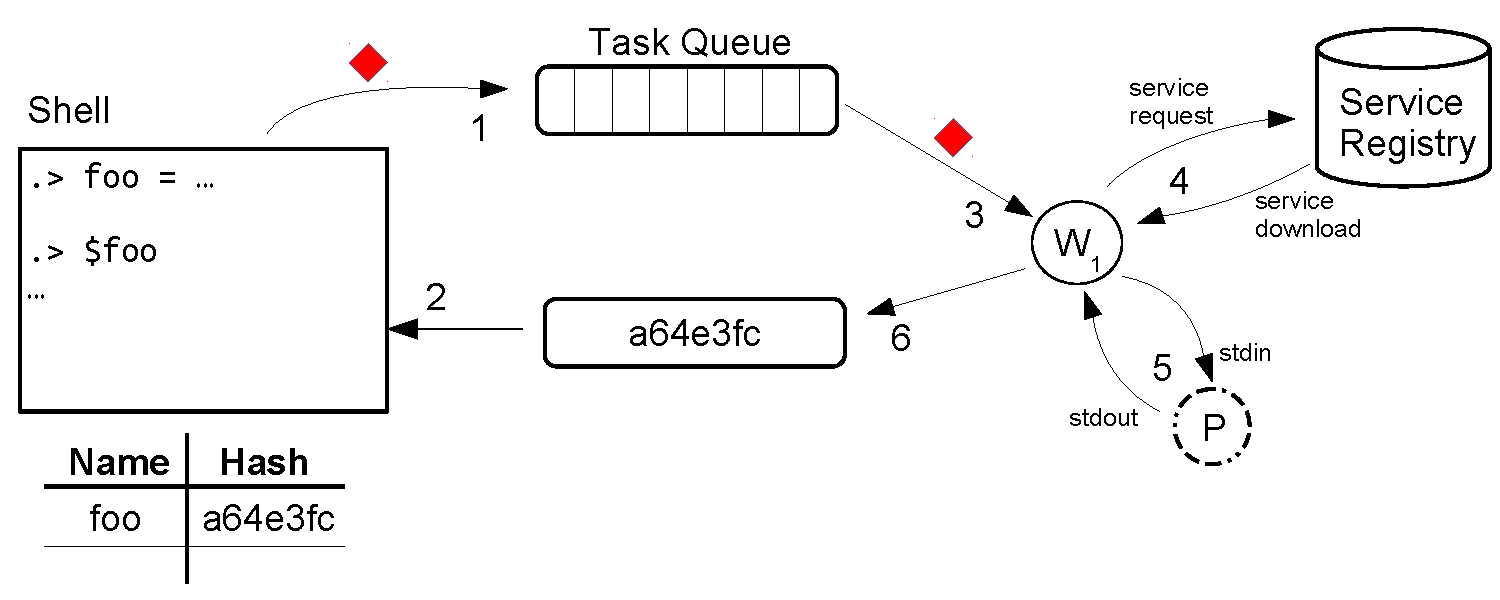
\includegraphics[scale=0.63, keepaspectratio]{system2.pdf}
  \caption{Detailed steps for processing a single task.}
  \label{system2}
\end{figure}

The command is then parsed and the task description structure
is created. If the command includes any already existing names,
the name table is used to resolve these names to their global
hashes. When the task description structure is finished, its
hash is stored in the name table behind the name \textit{foo},
as shown in the example.

Since names that are used in the command are first resolved to
their global hash names, it means that the final hash for the
task is calculated over a structure that might already contain
other hashes. Therefor the resulting hash might be a hash of hashes
and tasks issued may form a \textit{Merkle Tree} \cite{merkletree},
\cite{merkletreewiki}, in the same way that the objects stored
by \textit{Git} in its underlying file system form such a tree,
as was discussed in chapter \ref{git}.
\newline

The task is then send to the task queue, which is shown as step
1 in Fig.\ref{system2}. If the command of the user contained the
pipe operator, the shell will split the chain up into individual
commands and replace the input names of each command with the
result hash of the task description structure of its
predecessor. The individual tasks are then send to the task
queue in the order in which they are read, from left to right.
Otherwise it would be possible to construct task chaines with
more tasks then available workers, which would bring the system
to a halt.

The task queue is implemented
as a \textit{RabbitMQ} message queue \cite{rabbitmq},
\cite{rabbitmqwiki}, \cite{rabbitmqbook}. It's important to
note that the current implementation uses RabbitMQ in the
version 3.6.6-1 and that RabbitMQ is run in the fault tolerance
and distributed mode, which means that queues are replicated three
times and messages are \textit{not} written to disk but rather kept in
RAM at all times. These fault-tolerance and scalability measures
are provided by the RabbitMQ message broker by default and were
used without any modifications except for configurations and
setup.
\newline

Since the result of the command is bound to a name, a new
prompt is immediately available to the user. It is now assumed,
for the sake of the example, that the user immediately wants to
see the data of the result and therefor queries the name
\textit{foo} using the query operator \texttt{\$}. This is
shown as step 2 in Fig.\ref{system2}. This showcases another
feature that is widely adopted by most message queueing
frameworks and infrastructure: both, consumer and producer,
are able to create queues. That means that whoever requests
a queue first, will trigger its creation and any subsequent
request for queue creation are being ignored as idempotent
by the message broker. So in this case it is assumed that
the shell, as the consumer, is first to request data from the
queue with the name \texttt{a64e3fc}. For step 2 it is further
assumed that no data is currently available, so no data is
printed to the user and the shell blocks in a sort of
receive loop, in the same that an actor would block, waiting
for new messages, as was introduced in chapter \ref{actorModel}.
\newline

Step 3 shows how the free worker $W_{1}$ receives the task from
the task queue. As will later be discussed in the error model
section, there is no spreading or redundant execution used in
order to deal with possible worker failure. A task must only
be received by a single worker and must also only be executed
\textit{exactly once}. This is another invariant of the system.
Guaranteeing that only exactly one worker receives a task
from the task queue is again already taken care of by RabbitMQ out
of the box. The internal queue scheduler used by RabbitMQ
uses round-robin scheduling by default. Therefor a new task
is only sent to exactly one worker. If that one fails, another
different worker will receive the task. A task is only ever
worked at by exactly one worker at a time.

The worker itself has no idea about the possible services
that are available in the system. The worker has been implemented
as a \textit{generic} worker. This means that the worker downloads
the service that is being contained in the task description from
the service registry and simply executes the received service, as
is demonstrated by step 4.

Since the generic worker is currently also written in Java,
the downloaded service could also just be Java code and therefor
executed by the worker instance natively. However, for the sake
of the example it is assumed that the downloaded service code
contains instructions to fork another Linux process. This means
that arbitrary executables can be executed by the worker, in
the same way that the foreign function interface of Cuneiform
allows to execute already existing bioinformatic tools without
any code modifications, as was introduced in chapter \ref{cuneiform}.
However, it needs to be said, that the current implementation
assumes that the binaries referenced are
already pre-installed on the worker node. However, this could be
easily avoided by also storing the needed executable in the service
registry and downloading it if necessary.
\newline

Step 5 shows how the worker has forked another Linux process.
The \textit{stdin} and \textit{stdout} (and \textit{stderr})
channels of the spawned process are redirected by the worker.
This allows the worker to receive any needed input from other
data queues in the system and forward them to the forked process
and receive any output of the forked process and forward this
output to the output queue of the worker and therefor the output
queue of the task. The forked process at no point needs to know
that it's being part of a distributed system of workers and
distributed message queues. This means already existing tools
can be re-used without any modification.
Step 6 shows how the worker forwards any piece of data
received from the forked process to the output queue, whose
name is the hash of the task description the worker received
in step 3. Whenever the worker produces an output data token,
anyone listening on this particular output queue will be able
to observe the data and so naturally the shell, as one such
listener would print the received data to screen.
\newline

Unfortunately there is a problem. Fig.\ref{system3} shows an
example including a data dependency between the task whose
result is stored behind the name \texttt{bar} and the task
whose result is stored behind the name \texttt{foo} because
the service \texttt{Cat} takes the data from \texttt{foo}
as input. Given the eager-evaluation of the shell, however,
there are multiple timings in which these
tasks might be invoked.

One would assume that the easiest one would be for the user
to take a break after she issued the \texttt{foo} command and
start the \texttt{bar} command only after the \texttt{foo}
has already finished and produced all its output data.
Then all the data would be ready even before the second task
is started, which could result in the same worker executing
both tasks. Unfortunately this is the most problematic case.

The ``best'' case in terms of implementing the data layer
using message queues only would actually be if the user
issued both commands immediately and the consuming worker,
worker $W_{2}$, was already consuming before the first data
item produced by $W_{1}$ arrived in queue \texttt{a64e3fc}.

\begin{figure}[h]
  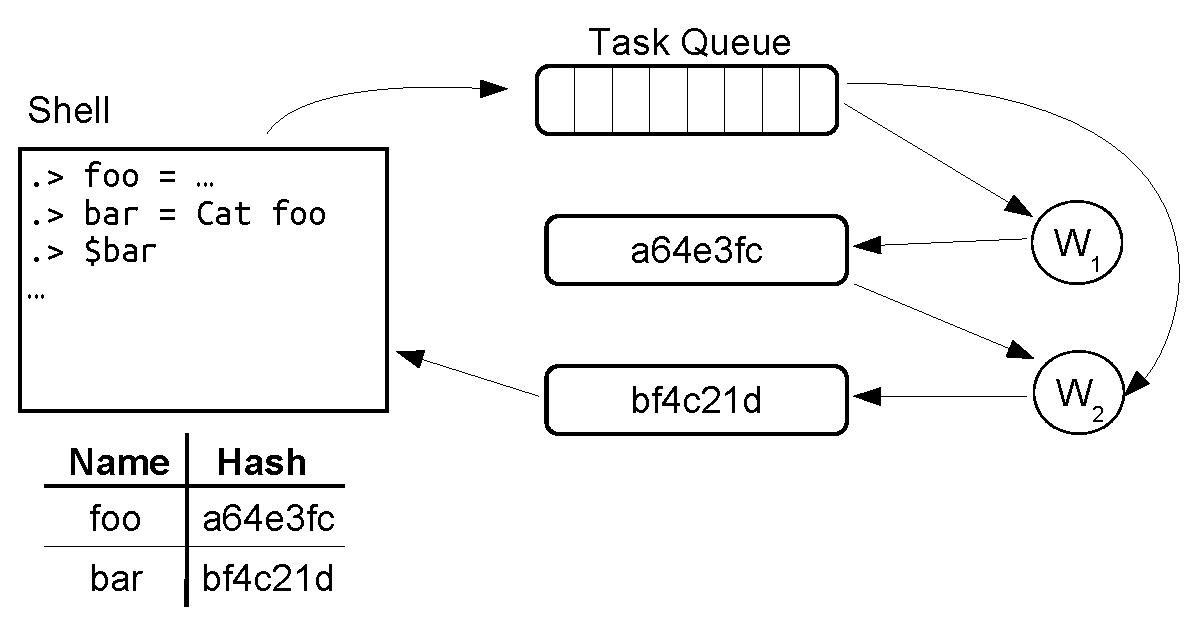
\includegraphics[scale=0.63, keepaspectratio]{system3.pdf}
  \caption{Example showing the data dependency between tasks.}
  \label{system3}
\end{figure}

This is due to the \textit{Abstract Message Queue Protocol}
(AMQP) which is implementing by almost all message queue
implementations and frameworks. The AMQP defines that,
although messages can be fanned out to multiple consumers,
a consumer only receives those messages that arrived in the
queue \textit{after} he registered at the queue, in the
same way that a chat client only receives the chat messages
that are posted, after it joined the chat room.

Since RabbitMQ implements the AMQP, it would've been impossible
to implement the data layer using RabbitMQ only, given the
eager-evaluation strategy of the Drift language because as was
described earlier, it must be possible for consumers to pull
data from a queue \textit{after} that data has already been
produced to that queue. In fact, consumers need to be able
to start consuming from the beginning of the queue, no matter
how much messages are already contained in that queue.

Luckily there is a new open source message queue project called
\textit{Apache Kafka} which does \textit{not} implement the AMQP
\cite{kafka}, \cite{kafkapaper}, \cite{kafkabook}.
Therefor Kafka queues keep their messages for a configurable
retention period, regardless of how many consumers ``consume''
them. It is debatable whether or not messages are still being
\textit{consumed} when they are not actually removed from the
queue. Therefor it is also possible to describe the service of
Apache Kafka as a distributed log, since messages pile up in
the queues without ever being deleted if the retention period
is set to infinity as was done in the current implementation.
\newline

Because messages that have been produced to a Kafka queue are
never deleted, it is possible for a consumer to connect to a queue
that already contains messages and read the messages in the order
of their arrival, starting from the very first messages. One could
say that the consumer can read the message \textit{history} of a
queue, in the same way that \textit{Datomic} allows the accretion
of facts to build up history, as was introduced in chapter \ref{datomic}.

\begin{wrapfigure}{l}{0.5\textwidth}
  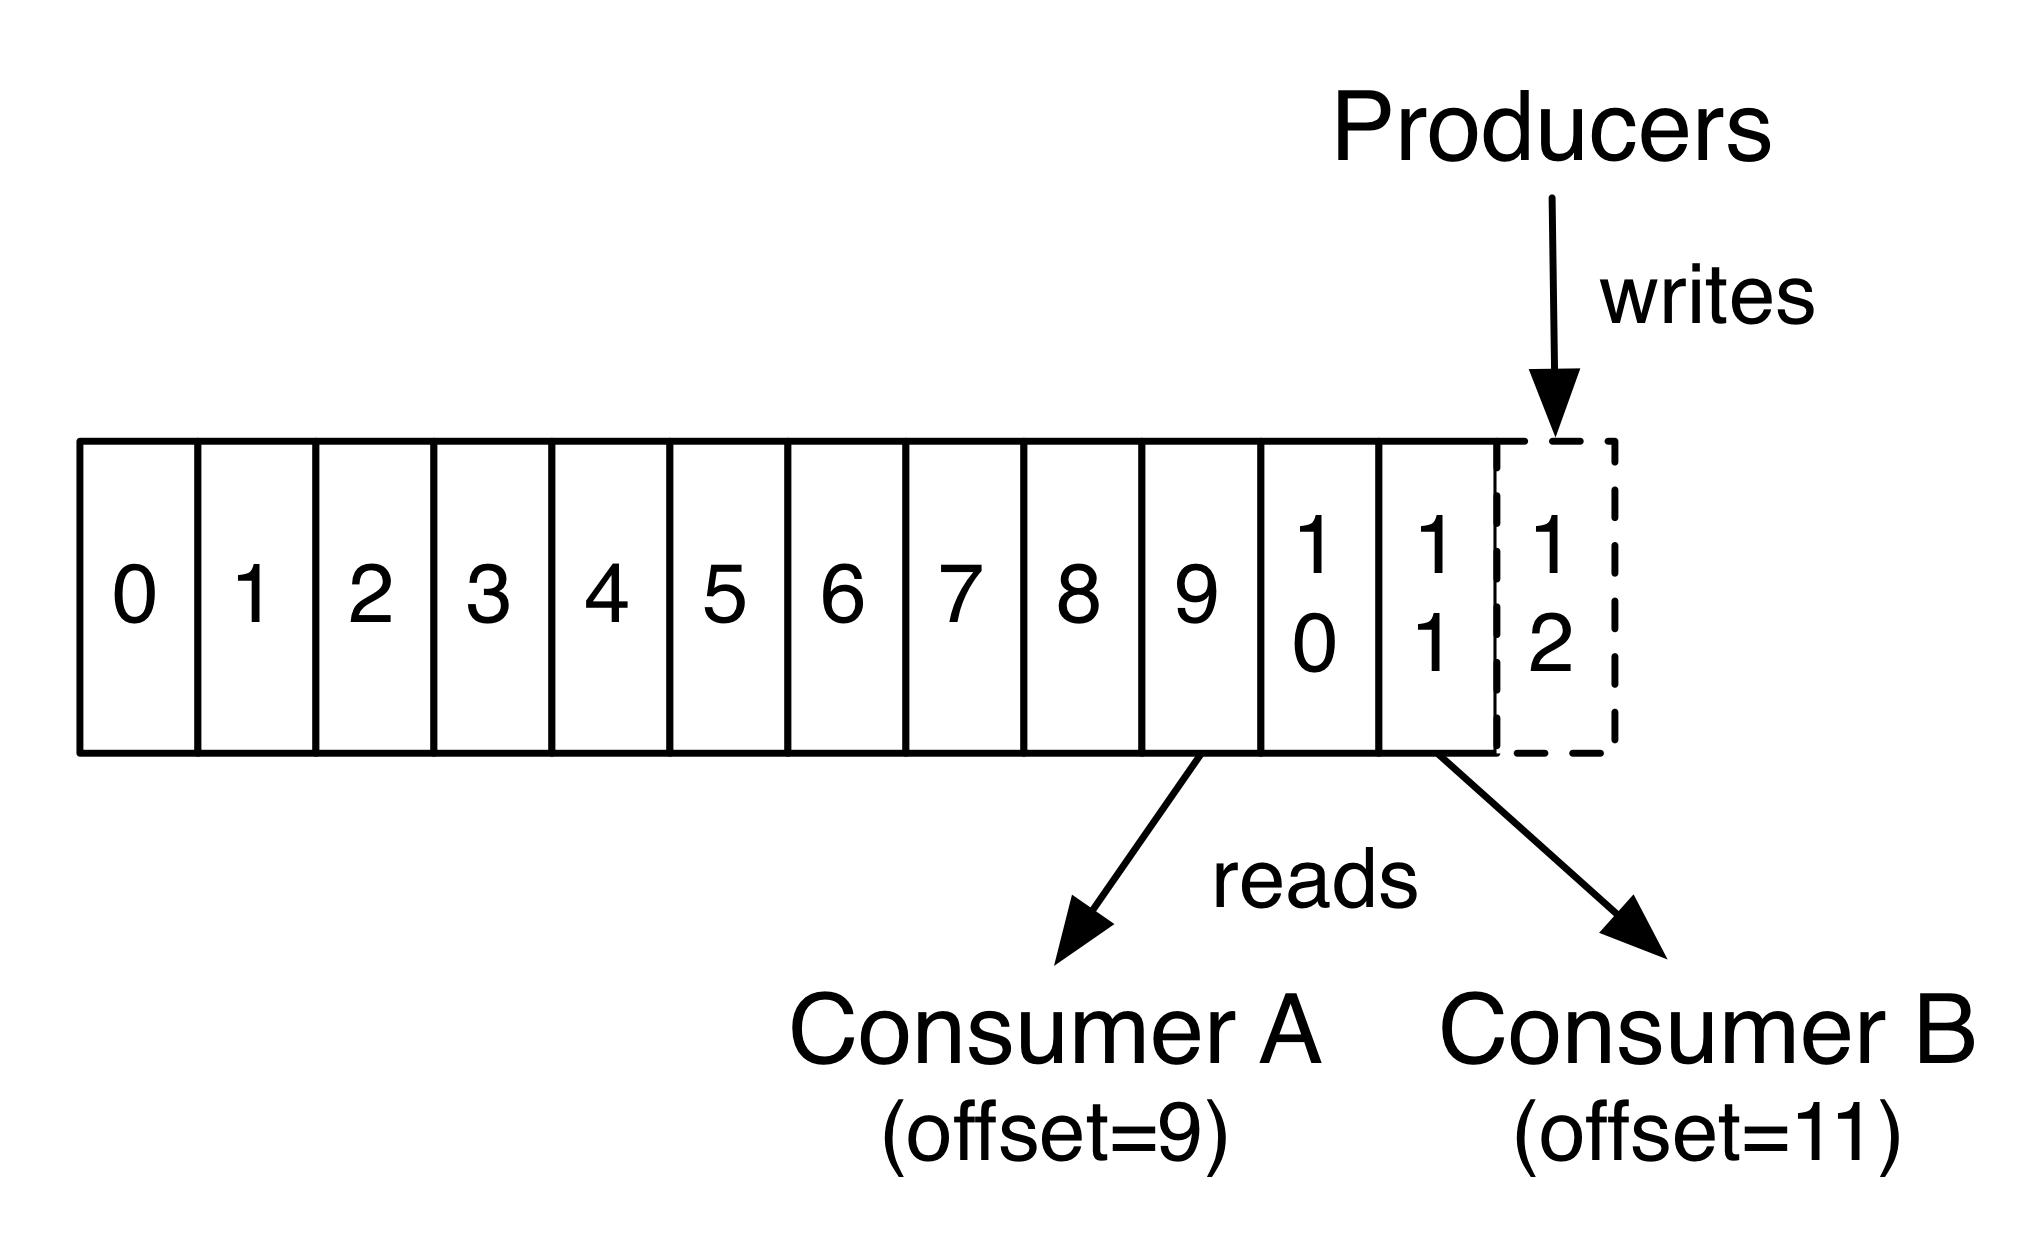
\includegraphics[scale=0.8, keepaspectratio]{kafka_consumers.png}
  \caption{Example showing multiple consumers independently reading from
           the same Apache Kafka queue at different positions.}
  \label{kafka-consumers}
\end{wrapfigure}

Furthermore, this \textit{immutability} of the messages allows
for multiple consumers to read and consume from the same queue
\textit{concurrently}, as shown in Fig.\ref{kafka-consumers} which
was taken from \cite{kafka}.
In RabbitMQ and other message queues that
implement the AMQP consumers are actually contending for messages
if they are consuming from the exact same queue. A fan out behavior
is also possible, this however needs all the consumers to have already
registered at the fan out component (which is called \textit{Exchange}
in RabbitMQ) before messages are being produced.
In Kafka any consumer can start consuming whenever he likes at
whatever position or message in the queue and completely unaffected
by any other consumer. Therefor the actual \textit{data queues}
in the Drift system implementation are Apache Kafka queues.

Because of this immutability and message store rather
than message queue nature, Kafka implements a \textit{pull-model}
instead of a \textit{push-model} as used by other message queues
like RabbitMQ. This pull-model has the client starting at a
specified message index called \textit{offset} and then pull
for new messages for a specified duration. When the poll
duration is over, the poll returns all messages that could be
fetched during the poll as a batch.

The current Drift implementation uses the Kafa Java API in
version \texttt{0.10.2}.
Unfortunately even in this latest Kafka version, the polling for data is
also used to also signal consumer liveness to the Kafka broker.
Kafka therefor effectively multiplexes the data channel (polling for data)
with the signal channel (liveness via heartbeats), resulting
in the consumer having to constantly repoll in order to not
be marked as disconnected by the Kafka server.
This is still true even when the queue the consumer is polling
on is \textit{deleted} using the external admin tool provided
by Kafka. Therefor an already ongoing poll is \textit{not}
interrupted by the queue deletion and any subsequent poll will
recreate the queue because consumers can also create queues
as was explained earlier. So any external \textit{problem}
with a queue must be signaled to consumers via messages inside
the queue. The only exception that can currently be used to
interrupt poll is a so called \texttt{WakeupExecption} which
must be thrown using the \texttt{Kafka.Consumer} object itself,
by another thread from inside the consumer.
\newline

This is implemented differently in RabbitMQ. Since RabbitMQ
implements the push-model, the user specifies callback methods
which are invoked whenever a message is delivered to the
consumer and this callback interface also allows to specify
a method which is triggered whenever the queue on which the
consumer is currently waiting for messages is deleted.
A single delete-action on a queue will trigger the delete
callbacks on \textit{all} consumers currently listening for
messages on that queue.

Therefor a single logical queue as used by the Drift
system always uses both: an Apache Kafka queue for the plain
data and a RabbitMQ queue for signaling any errors to all
consumers.

\begin{figure}[h]
  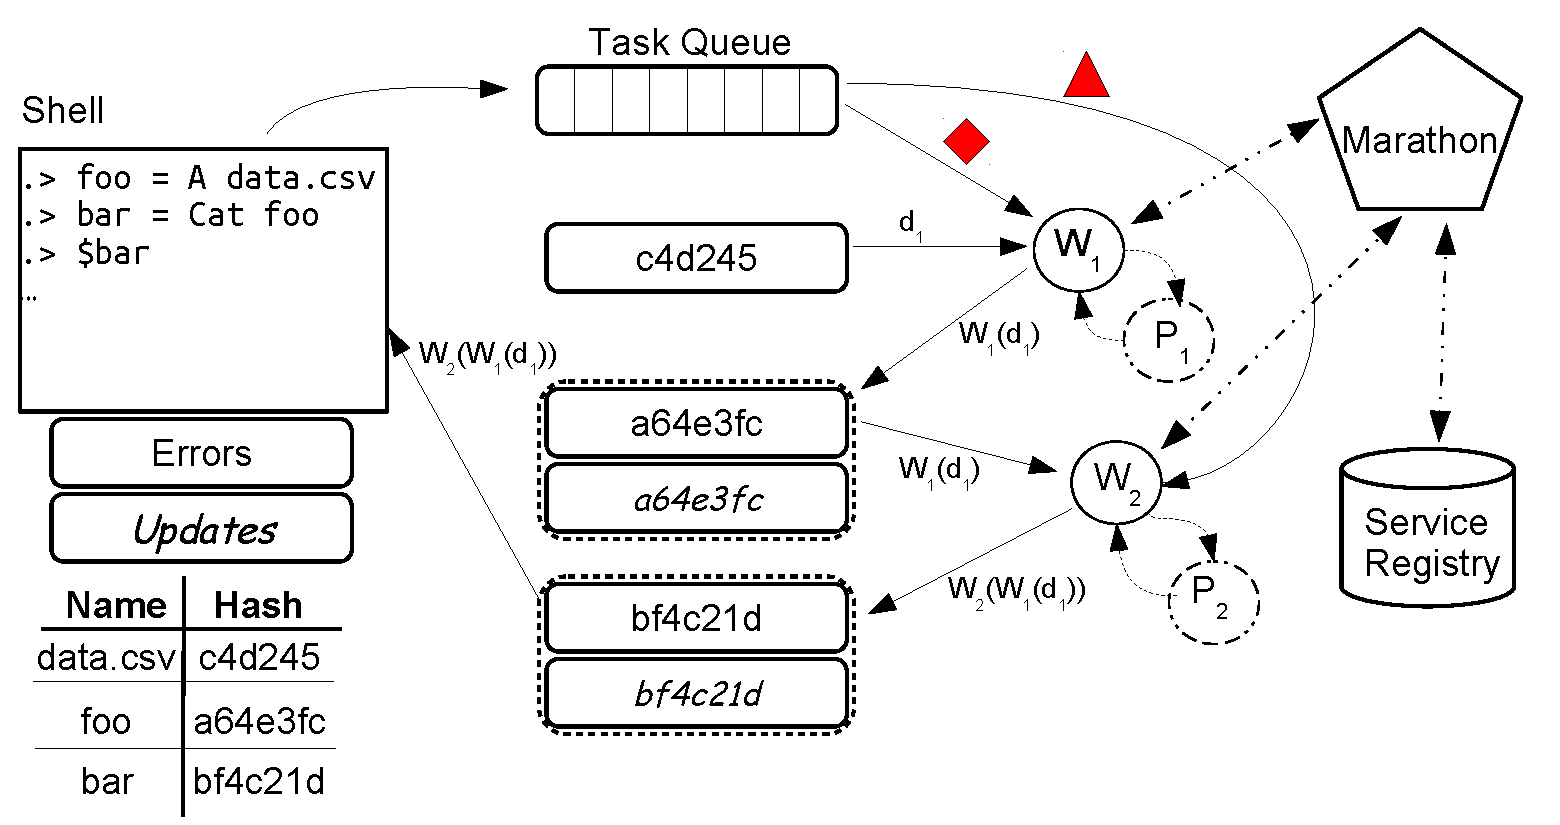
\includegraphics[scale=0.63, keepaspectratio]{system4.pdf}
  \caption{Example showing the full extent of the Drift back end.
           Two workers are running, forming a data dependency with
           one worker consuming from a data queue created by an import
           and the other working consuming from the output data queue
           of the first worker.}
  \label{system4}
\end{figure}

Fig.\ref{system4} tries to illustrate the full extent of the
Drift back end. It shows two workers forming a data dependency.
The first worker, $W_{1}$, received the diamond task which specified
to consume from the input queue \texttt{c4d245}. Since this is only
a single data queue, this represent data that was once imported
because of the import either failing or succeeding there is no need
any further signal queue for intermediate task failure. The data queues
(Kafka queues) are named with normal letters whereas the signal
queues (RabbitMQ queues) are named with italic letters.

After having downloaded the required service from the service registry,
worker $W_{1}$ spawns another Linux process $P_{1}$
as specified by the command it received. It then forwards any data
item it received from the input data queue to this process and
any data item produced by the process to its output data queue.
Worker $W_{2}$ does exactly the same independent of $W_{1}$.
It receives the triangle command, downloads the required service and
spawns the service as a new Linux process. The triangle command
contained the hash \texttt{a64e3fc} as an input queue for
$W_{2}$, so therefor $W_{2}$ consumes from the ouput queue of $W_{1}$
and produces to its output queue, whose name is the hash of the
command structure that already contained the hash of the output queue
of $W_{1}$, as was explained earlier. Since the user queries the
result of \texttt{bar} and not the result of \texttt{foo}, the shell
then consumes from the output queue of $W_{2}$ and shows every data
item received to the user.
\newline

The examples so far have shown the detailed execution of services
dealing only with regular data which is either bound to
a single name and then later queried by the user or directly
printed to the screen when received by the shell. But as was
introduced in chapter \ref{driftlang} there are also tasks that
receive or produce a \textit{namespace}.

\begin{figure}[h]
  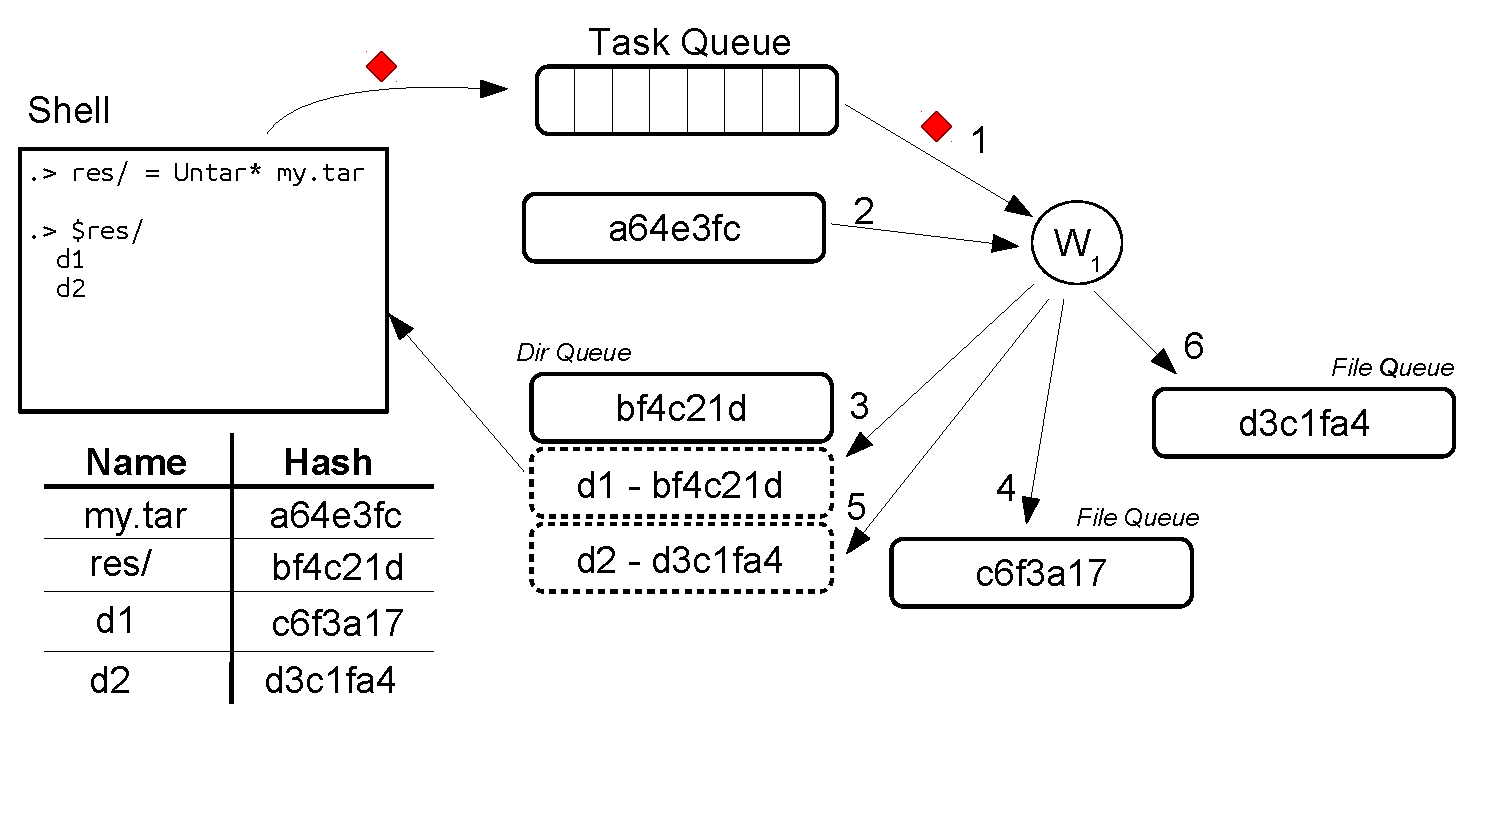
\includegraphics[scale=0.63, keepaspectratio]{dirqueue.pdf}
  \caption{Example showing the creation of a namespace using
           directory queues that contain the original file name
           and their hash name and the actual data queues representing
           files.}
  \label{dirqueue}
\end{figure}

Figure \ref{dirqueue} shows how the creation of a namespace
is implemented by the Drift back end. As can be seen the user
issues the \texttt{Untar*} command that was already introduced
earlier. The asterix on the right side of the command name
indicates that it produces a namespace and therefor
its result must also be bound to a namespace, as indicated by
the \texttt{/} in the name \texttt{res/}.

After commiting the task to the task queue the shell inserts
its hash into its name table, so the namespace \texttt{res/}
is listed by \texttt{ls} and is also queriable. Querying a
namespace results in effectively querying what is called the
\textit{directory queue}, because of the close resemblance of
names and namespaces to directories and files in the original
UNIX file system.

The worker receives the task, which is shown as step $1$,
and then receives its input data from the appropriate queue,
namely the queue that contains the \texttt{.tar} file which
that was created by an import as indicated by the name. This
is shown as step $2$.
Now for every resulting name in the namespace the worker will
first \textit{publish} its name and its hash to the directory
queue with the hash being again the content hash of the extracted
file in the case of \texttt{Untar*}. Therefor the this name would
now be available as a name inside the \texttt{res/} namespace
in the shell and could be used for further commands. This is shown
as step $3$ in Fig.\ref{dirqueue}. The worker
will then start to fill the data queue of the published name which
is step $4$.
When it finished the first name, it will publish the next name
and start filling its data queue until every name in the namespace
has been created, which is illustrated by step $5$ and $6$
\footnote{In this example the dashed queues do \textit{not} represent any
signal queues but are just supposed to illustrate the entries
of the directory queue.}.

So therefor not only the data behind names is streamed, but also
the content of namespaces is stream as well as the data behind the
names contained in that namespace.
\newline

Going back to the full back end overview as shown in Fig.\ref{system4},
a new element besides the already introduced \textit{Service Registry}
is shown, namely \textit{Mesos Marathon} \cite{marathon}.
Marathon is a distributed
fault tolerant watch dog process that monitors services spawned
through its interface. If a failure of such a process is detected
by Marathon, the failed service gets restarted without any further
effort by the programmer or system administrator. Marathon is one
component of the \textit{Mesosphere} project which started out
as a distributed resource negotiator called \textit{Apache Mesos},
which is now it's probably most widely known component
\cite{mesosphere}, \cite{mesos}. Since Marathon monitors
Mesos containers, the workers as well as the service registry are
executed as Mesos containers.
\newline

So therefor all of the core components of the back end, both message
queue frameworks including the task queue and Marathon are run in
distributed mode. That means that the message queues are automatically
replicated three times and keep all their messages \textit{only} in RAM.
Disks are never used. Marathon itself is also replicated three times
with one master and two slaves in order to provide fault tolerance.

It's important to note that these are the fault tolerance capabilities
that these tools offer by default. Apache Kafka for instance comes
with its own Apache ZooKeeper instance for internal distributed
coordination and distributed consensus that itself is also run in
distributed mode, meaning being replicated amongst multiple nodes
\cite{zk}, \cite{zkpaper}.

\begin{wrapfigure}{l}{0.5\textwidth}
  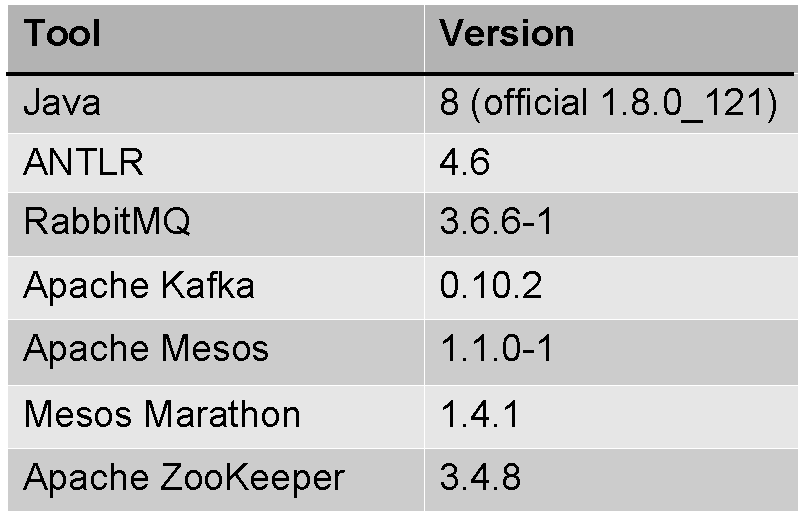
\includegraphics[scale=0.6, keepaspectratio]{toolstable.pdf}
  \caption{Overview over the tools and their versions as used
           in the current implementation.}
  \label{toolstable}
  \vspace{-10pt}
\end{wrapfigure}

Although all of the used tools are open source software, with their
code being freely available via \textit{Github}, all these tools were
used without any code modifications. Therefor most of the fundamental
problems of programming a distributed system, like distributed
messaging or distributed consensus are being taken care off.
The main challenge therefor lies \textit{not} in resolving these
already solved problems but rather in learning how to utilize
these tools given the vast variety of tools, options, configurations
and customizations.
Fig.\ref{toolstable} summarizes all the tools and their versions
as used by the current implementation.

\subsubsection{Error Model}
\label{errormodel}

Since now that all of the components of the Drift back end have
been introduced, the last thing that needs to be discussed is
the handling of errors. The basic failure model that is assumed
for the components of the back end (the system) is
\textit{crash-recovery}. This is realized by using Mesos Marathon
for spawning, monitoring and restarting the worker processes and
the service registry. The used message queues again offer the
restarting of lost queues out of the box.

Before introducing the error cases, Fig.\ref{system5} shows
the normal mode of operation. This uses the same example as
was shown earlier, omitting the unnecessary parts. So again
one can see the two tasks $W_{1}$ and $W_{2}$ processing
what has been bound by the user to the names \texttt{foo} and
\texttt{bar} respectively.

\begin{figure}[h]
  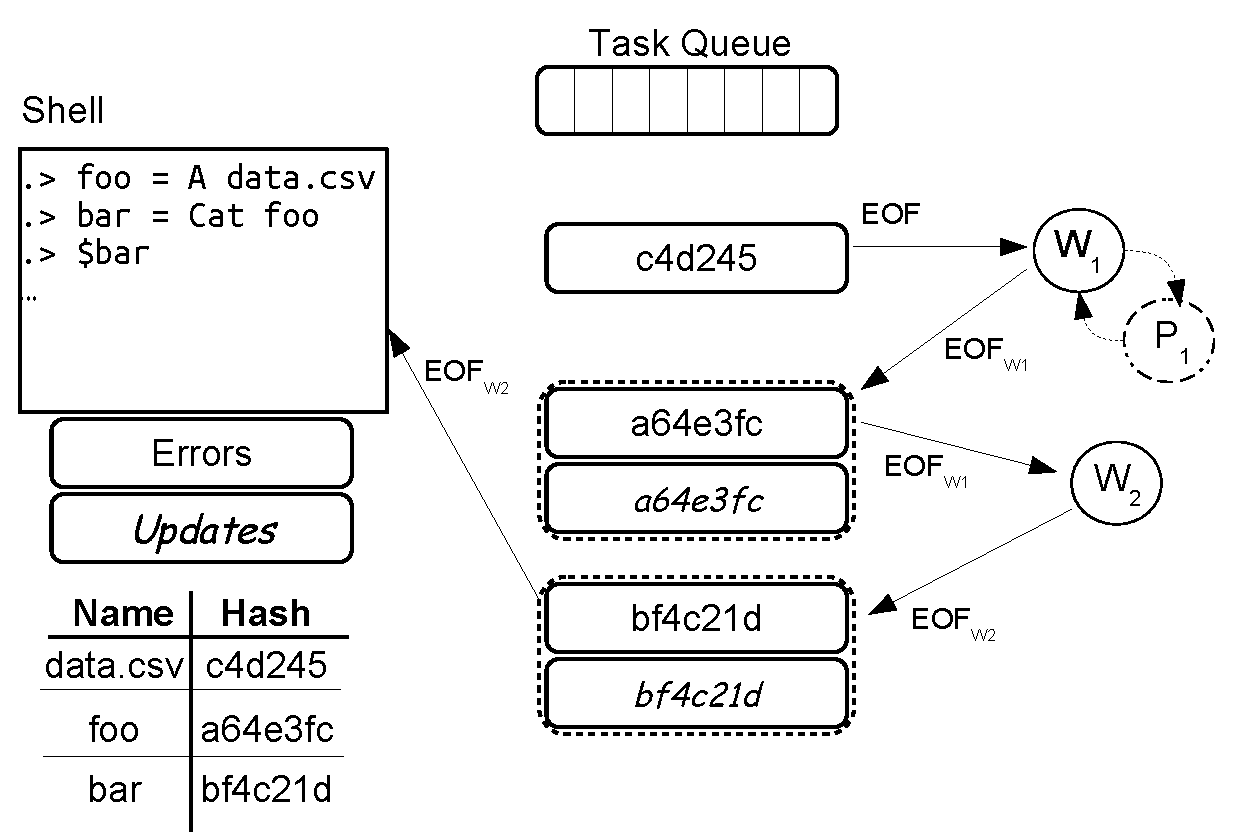
\includegraphics[scale=0.63, keepaspectratio]{system5.pdf}
  \caption{Example showing the successful completion of two
           tasks and the propagation of the \texttt{EOF} token.}
  \label{system5}
\end{figure}

Worker $W_{1}$ consumes its input from a data queue which was
created by importing a local file. After the import has finished,
the import action itself inserts a special coordination token,
an \texttt{EOF} token, into the data stream. When worker
$W_{1}$ has consumed all the data token available in this
input queue, he will consume the \texttt{EOF} token. This
signals the end of the input data stream and triggers the
termination of the spawned process $P_{1}$. After the process has
been gracefully terminated, $W_{1}$ also sends an \texttt{EOF}
token to its own output queue and starts listening for new
tasks at the task queue again. Therefor, naturally, whenever
$W_{2}$ or any other consumer reaches the end of the data
stream produced by $W_{1}$, it will encounter the \texttt{EOF}
token of this stream which again triggers the creation
of its own \texttt{EOF} token.

This \texttt{EOF} mechanism is of course also used when
dealing with the creation of namespaces and therefor
directory queues, as for example shown in Fig.\ref{dirqueue}.
Each individual name will be finished by inserting the \texttt{EOF}
token into its data queue and at last the worker will finish
up the directory queue by also inserting the \texttt{EOF} token.
\newline

This showcases an important overall property of the Drift back end
implementation: the only thing that \textit{any} worker needs
to know is only its immediate environement, i.e. where to read its
input from and where to produce its output to. If a worker
is finished, it closes its ouput stream by producing a last
\texttt{EOF} token, without having any idea whatsoever about
who or how many other workers might wait for the next token
and without any global knowledge about the overall
data dependency graph built up by the user.

This is heavily inspired by \textit{Petri Nets}, a theoretical
model for describing distributed systems \cite{pnbook}, \cite{pnwiki}.
The core concepts of Petri Nets are \textit{places}, literally
places where tokens can reside and \textit{transitions}, actions
that consume tokens from their input places and produce tokens
to their output places. The relevant aspect of Petri Nets is that
whether or not a transition is \textit{enabled} (can fire) only
depends on the number of tokens on all of its input places.
Therefor each and every transition is enabled independent of
any other transition and carries \textit{no} global knowledge about
the net it is being part of or any other global state which is
the key property for scalability in the context of distributed
systems.

In that same spirit, every worker in the Drift system has no
idea about the overall structure of the system or the complexity
of the data dependency tree that was and is being created by the
user. Every worker directly consumes from the inputs contained
in the task description and produces to an output queue named after
the hash of the task description itself.

Therefor, when the \texttt{EOF} token is produced by one worker, it will
slowly but definitely trickle down whatever data dependency tree
has been created by the user. Reaching every listening worker
without ever knowing about them. Every listener will then create
its own \texttt{EOF} token, therefor propagating the token one
level further down the dependency tree.
\newline

Given the invariant of the system that service invocations are
\textit{deterministic} and using the described setup, the system
differentiates between two error cases: either a \textit{system failure}
or a \textit{user failure}.

A user failure is encountered whenever a task issued by the user
made it to the task queue but leads to an error when it is finally
executed by the worker. For instance this could be case whenever
the user issues a command in which a service consumes some input
but the process that is spawns expects a different input format
as provided by the input queue specified by the user. Naturally
this will lead to an error produced by the forked process and
will result in the cancelation of the task.

Unfortunately these types of errors, the user errors, cannot be
resolved by the system. Under the assumption and system invariant
that tasks are deterministic, it holds that a task that led to
a processing error, will recreate the same error if executed again.
Therefor restarting the task using a different worker would only
lead to the same error result. Therefor the whole task needs to
be marked as erroneous and to do that the worker will produce
the only other special control token besides the \texttt{EOF} token,
a \texttt{ERR} token. This \texttt{ERR} token is inserted into the
output data queue of the task and the worker will signal the task
completion to the task queue, so no other worker will receive
that task. Therefor the error result is forever persisted with
this specific task invocation.

Interestingly, if the error only happened \textit{after} some
resulting data tokens were produced by the task, the error token
is only added to the output stream. This means that no further data
will be added to the ouput, but the data that was produced before the
error occured can still be consumed from the queue until the
\texttt{ERR} token is reached.

if a consuming task reads the error token from at least on of
its input queues it will gracefully terminate its own processing
and produce its own \texttt{ERR} to its own output queue accordingly.
Therefor a single error will slowly but definitely propagate through
the whole dependency tree, in the same way the \texttt{EOF} token
is propagated, as was shown in Fig.\ref{system5}.

Additionally any worker who encounters an error, whether produced
by its own processing or by consuming the \texttt{ERR} token from
one of its inputs, will produce an error notification to the
\texttt{Errors} queue. This queue is read by the shell in a
seperate thread which then marks and updates the names managed by the
shells internal name table to indicate that certain names
resulted in an error. This is done to prevent the user to issue
commands including names for which it is already known that they
resulted in an user error. So if a name is used for which this
information is already contained in the \texttt{Errors} queue,
the command will be blocked and an appropriate error message is
displayed to the user.

Again, it's important to note that because of the eager-evaluation
and immediate feedback strategy of the Drift language and therefor
its shell, it is possible that the users issues a command which contains
a task that will soon encounter an error, or maybe even has already
encountered an error but the information, the message itself, has
not yet reached the \texttt{Errors} queue or is just being processed
by the shell. So the task will be send, will be executed and then
encounter the \texttt{ERR} token in one of its input streams just
as described earlier.

The data a task produced before it might encountered an error is
kept, in order for the user to be able to inspect what might have
gone wrong. So eventhough the user cannot use the erroneous name
besides overwriting it with a new command, she can always
query the faulty name and the data available behind that name will
be printed by the shell until the \texttt{ERR} token is reached.

Since task invocations in terms of user failure have this
all-or-nothing property, because of the task determinism invariant,
dealing with such errors is actually straight forward.
The other class of errors, the system failures, are actually a bit more
involved and are the reason why each Kafka data queue is mirrored
by a RabbitMQ signal queue.
\newline

The error category of \textit{system failures} encompasses anything
related to the execution of the workers or the distributed message
queues. This means crashing, running out of disc space, memory or
any other form of resource or simply not being reachable via the network.
It is thought of being the responsibility of the system administrator
to fix such errors in terms of providing the necessary hardware.
Any software monitoring and restarting as well as replicating is either
done by Marathon in case of the workers and service registry or in
case of the in-memory messages handled by the distributed message
queue brokers themselves.

Since the user is not supposed to deal with those kind of failures
it wouldn't make sense to present them to the user in any form.
Therefor it is another invariant of the system that the user should
never be able to recognize any form of system failure. Especially
not when observing data.
This is done as illustrated by Fig.\ref{error1}.

\begin{figure}[h]
  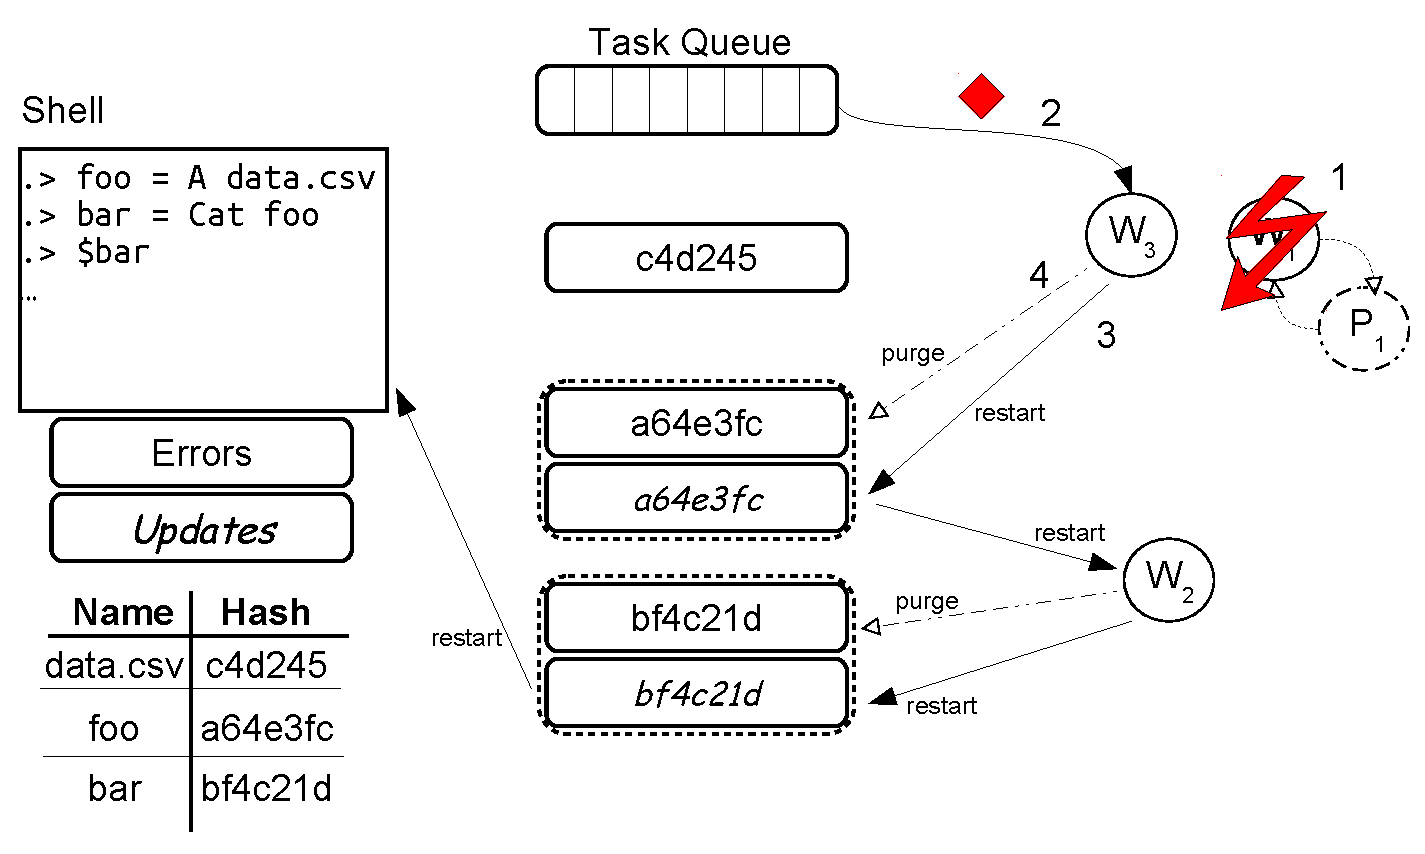
\includegraphics[scale=0.63, keepaspectratio]{error1.pdf}
  \caption{Example showing a worker crash and failover strategy
           including signal queue deletion and purging of the
           data queue.}
  \label{error1}
\end{figure}

When a worker crashes or is unable to
continue, it is assumed that any process it might have spawned
will also be terminated and therefor discontinued. This is shown
as step $1$ in the example.

Since the task queue (RabbitMQ broker) will have detected the
missing worker but did not receive a task completion notification,
it will redistribute the task to any other worker currently
ready to receive new tasks. In the example above this is worker
$W_{3}$ as shown by step $2$. Given the invariant of the system
that a task result must be presented as if this task has been
executed \textit{exactly-once}, any worker receiving a new task
first checks whether or not the expected result queue named after
the hash of the task description itself already exists.
Unfortunately this information alone is not enough. As was
explained earlier, any consumer could have also already triggered
the creation of said result queue by listening for data on it.
Although possible this is rarely the case in terms of other workers
given the order in which tasks are inserted into the task queue
and therefor producers and consumers are spawned but one must not
forget, that the shell is also considered a consumer.

Therefor it is possible that the shell is already waiting for
the result of a task for which the corresponding worker has
just received the task description. To account for that a worker
not only checks for the mere existence of the result queue but also
reads the last token that was produced to that queue. If that
token is not the \texttt{EOF} nor the \texttt{ERR} token, it inferes
that the task has already been started by another worker which
must have crashed.

The worker $W_{3}$ then starts the clean up process as illustrated
by step $3$ and $4$. It first \textit{deletes} the signal queue.
This will trigger an immediate notification and callback invocation
at \textit{every} listener without knowing them directly (steo $3$).
Then, it sets the retention period for the corresponding Kafka
data queue to the minimum value (step $4$). The Kafka broker has been
configured to aggressively poll any retention period change, so that any
retention period change will be carried out almost immediately
(in around 10 seconds). Lowering the retention period of a queue
to a couple of seconds, triggers the deletion of any message after
that duration. Therefor reducing the retention period to its minimum
value effectively purges the content of a queue which takes on average
about $60$ seconds even for large queues.
After sending the retention period change, $W_{3}$ will wait for
two minutes before restarting the execution of the task. That
means recreating the signal queue and spawning any necessary
process and resetting the retention period of the data queue to
infinity. It will then refill the data queue that now is assumed
empty.

Any worker that received the delete trigger via the signal queue
will do the same for its own signal and data output queue. That
means it will first delete its own output signal queue, purge
its output data queue, terminate its process and then wait for
two minutes before resetting the retention period of the data queue
and restarting the process.
Therefor the resetting also propagates through the whole dependency
tree without any component ever knowing its complete structure,
just as the \texttt{EOF} and \texttt{ERR} tokens propagated through
the network.
Admittedly, setting the retention period of the Kafka data queues
to its minimum value in order to delete already produced messages
before the crash seems like a hack. Unfortunately, given the
immutable nature of the design of the Kafka message queues, even
the newest version does not provide any mechanism for explicitly
deleting messages from queues.

This reset procedure assures, that when an \texttt{EOF} or
\texttt{ERR} token has been produced to a data queue, the content
of the data queue looks like as if the task that produced it
was only executed exactly once. This whole procedure is also
retried indefinitely because it is only triggered by system
failures and it is assumed that these are taken care of by
the system administrator as soon as possible.
\newline

However, there is one last problem. It is true that the final
result looks like the task that produced it was only executed once,
but the user could have queried the data queue at any intermediate
point in time, just when some data had already been produced
but the worker crashed. In order to hide the re-execution of a
task and refilling of the data queue after a restart from the user
another feature of Kafka message queues is used because
Kafka queues not only store plain messages but rather
\textit{key-value} pairs where the key can be chosen
by the producer and the value represents the actual message.

In the Drift system, the keys are managed by the corresponding
worker, who will increment the key for every insert into the
data queue. But the shell also retreives these keys whe
consuming messages that are then immediately printed to the
screen. So for example imagine a case in which the user queried
the result of on ongoing task, which has already produced three
output items, $a, b, c$ when the user issues the query.
The task is now about to produce its next output item $d$ and
suddenly crashes but $a, b$ and $c$ have already been printed
to the screen in the shell. The whole failover procedure that
was described above is triggered and so the data queue is resetting
meaning $a, b$ and $c$ are deleted. The shell however still waits
for the next new data item $d$. The next message it will receive
from the data queue however will be $a$ again, since the whole
task is restarted from scratch.


So instead of buffering already received messages and comparing
any new incoming messages with the already received ones, figuring
out which one have already been displayed and which haven't, the
shell simply stores the key of the last message that was printed
to the screen. Any message that is further received with any key
lower than that will be discarded. Only the data item with the
next highest key will be shown. Therefor observing the data
from the user perspective will always look like a single
continuous execution of the task.
\newline

The same approach is of course also used when dealing with system failures
during the creation of a namespace. Figure \ref{direrror} tries
to illustrate an error case based on the example shown in
Fig.\ref{dirqueue}.

\begin{figure}[h]
  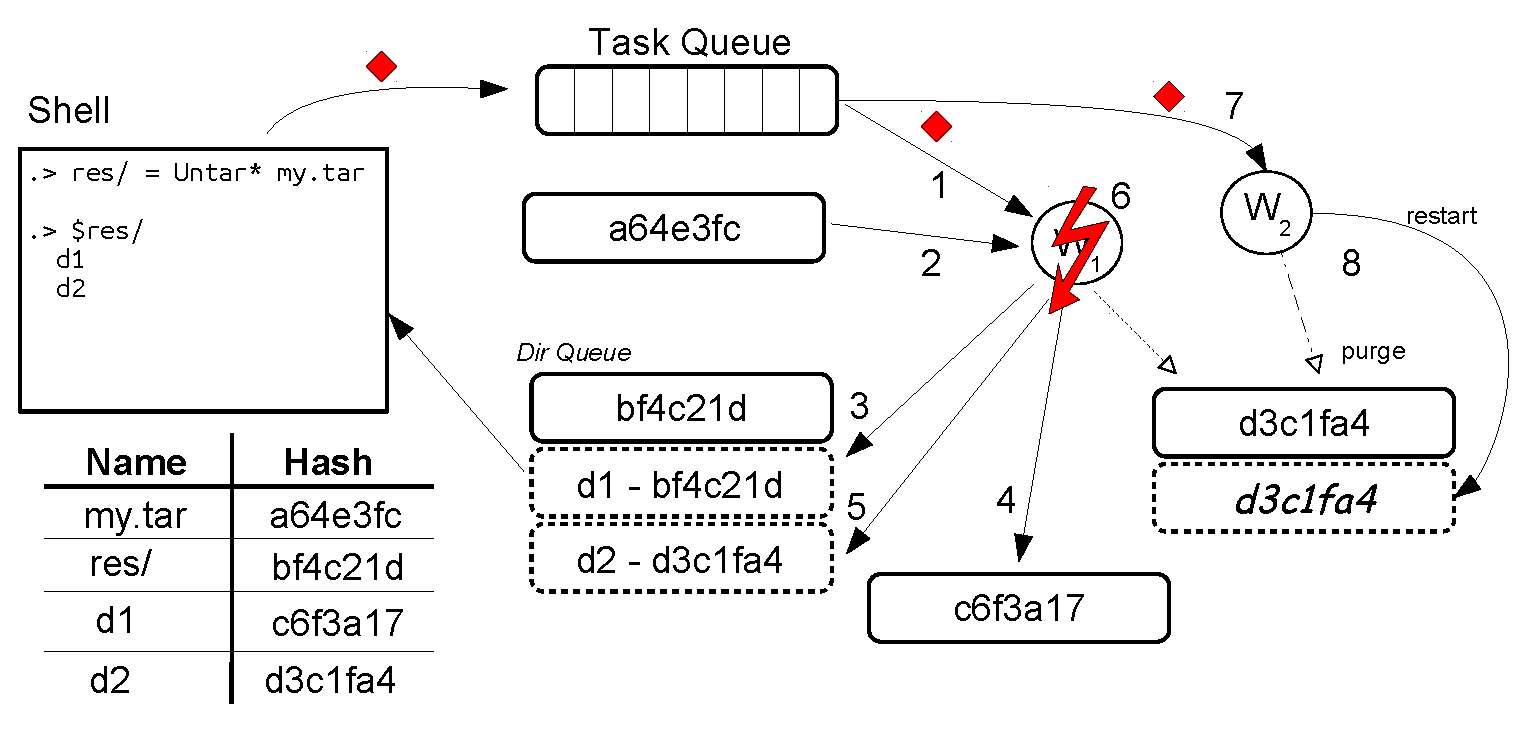
\includegraphics[scale=0.61, keepaspectratio]{direrror.pdf}
  \caption{Example showing the handling of a worker crash during
           the creation of a namespace.}
  \label{direrror}
\end{figure}

As was shown earlier, the worker $W_{1}$ first received the
\texttt{Untar*} task. It therefor received the \texttt{.tar} file
from its input queue and first published the name of the first
result name to the directory queue, making it available to
the user, before then uploading its content to its data queue,
as shown by steps 1-4. After finishing step 4 by inserting
the \texttt{EOF} token into the data queue of the first name, worker
$W_{1}$ published the next name to the directory queue and
started uploading its data to the appropriate queue. So now
it is possible that the user has already queried the content
of the second name in that namespace and has already been streamed
the first data items as they were produced by $W_{1}$.

It is now assumed for the sake of the example that $W_{1}$ crashes.
As already introduced Worker $W_{2}$ will
now receive the task and is supposed to finish the
namespace creation. So $W_{2}$ also pulls the input data
from the input queue specified in the task description but
instead of restarting the whole namespace creation process it
first checks the directory queue (whose name it can calculate
by hashing the task description it received) for any already
published names. For each name that has already been published
it then checks the last data item in that name's data queue.
If the last item is not an \texttt{EOF} or \texttt{ERR} token
it triggers the same reset-and-purge process that was already
introduced. Therefor each unfinished name is recreated from scratch,
which is again signaled to anyone listening on that name's queue.
But every name that was already finished by any worker that tried
to create that namespace before is left untouched.

Therefor the same mechanism is applied in the shell, which as was
assumed already queries the second name in the created namespace.
Only messages from that name's queue with a key higher than the
latest received key are shown to the user, therefor streaming a name
from a streamed namespace behaves exactly the same as dealing with
any other name.

\begin{wrapfigure}{l}{0.5\textwidth}
  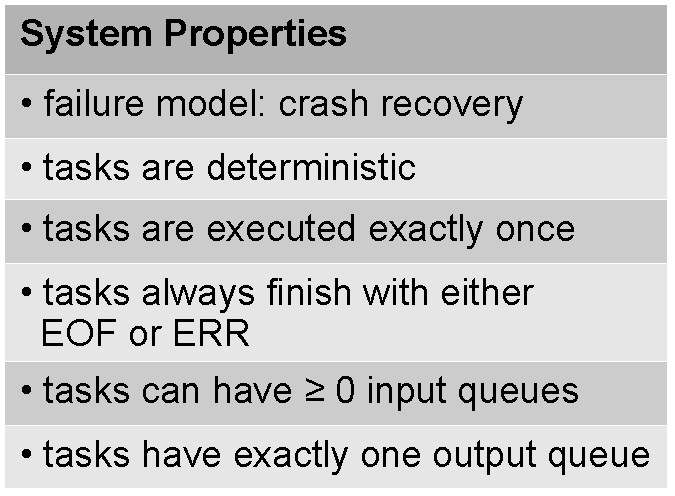
\includegraphics[scale=0.63, keepaspectratio]{invariants.pdf}
  \caption{Table summarizing the properties and invariants of
           the Drift system implementation.}
  \label{invariants}
\end{wrapfigure}

This concludes the handling of any system failures. As a side note
it should be mentioned that the final design of using the
\texttt{EOF} and \texttt{ERR} tokens as control tokens and inserting
them into the data stream was not at all obvious at the beginning.
Different designs were implemented that featured multiple Apache
ZooKeeper instances which allowed crashed workers to recover their
last state and continue where they crashed. Although these designs had
their advantages in terms of failover delay, the overall design
of the back end system became ever more complex and harder to
reason about. Using the control token approach all the used
ZooKeeper instances could be eliminated and the overall design
became much simpler.

The price that is being paid for that simplicity is that the
recomputation done by the failover worker restarts from scratch
by purging every item that had already been produced to the
resulting data queue. But given the overall and inherent complexity
of the distributed system context this price was deemed acceptable
because the recomputation can easily be further shortened as will
be explained in chapter \ref{futurework}.

Figure \ref{invariants} summarizes the system properties and
invariants of the current Drift back end implementation
that have been described so far.
\newline

The only thing that so far has been shown on in the examples
but not yet talked about is the \texttt{Update} queue, which
is for example shown in Fig.\ref{system5} and is implemented
as a RabbitMQ queue compared to the \texttt{Error} queue, a
Kafka queue.

The reason why the \texttt{Update} queue has not been introduced
yet is because it is mostly irrelevant to the overall back end
system implementation. Its sole purpose is to serve as an event
interface for any front end implementation like the Drift shell.
Any action that is undertaken by the back end system is sent as
an event to the \texttt{Update} queue. So whenever a worker
receives a new tasks, or finishes as task (with either \texttt{EOF}
or \texttt{ERR}) or restarts a task, it sends a short event
description to the \texttt{Update}. These can then be used
for example by any visual front ends to dynamically update the
visualization of the system that is shown to the user, as will
be described in the next chapter when the \textit{Drift UI} will
be introduced.









